\documentclass[11pt]{amsart}
\usepackage{geometry}                % See geometry.pdf to learn the layout options. There are lots.
\geometry{letterpaper}                   % ... or a4paper or a5paper or ... 
%\geometry{landscape}                % Activate for for rotated page geometry
%\usepackage[parfill]{parskip}    % Activate to begin paragraphs with an empty line rather than an indent
\usepackage{graphicx}
\usepackage{amssymb}
\usepackage{epstopdf}
\usepackage[usenames,dvipsnames]{color}
\usepackage{fancyvrb}
\usepackage{listings}
\usepackage{booktabs,footmisc}
\usepackage[colorlinks = true,
            linkcolor = black,
            urlcolor  = blue,
            citecolor = black,
            anchorcolor = blue]{hyperref}
\usepackage{hyperref}
\usepackage[all]{hypcap}

\usepackage{topcapt}
\usepackage[section] {placeins}
 
% include the lines below to use a nicer fixed-width font than the default one
 
\lstset{fancyvrb=true}
\lstset{
	basicstyle=\small\tt,
	identifierstyle=,
	commentstyle=\color{Bittersweet},
	stringstyle=\color{red},
	showstringspaces=false,
	tabsize=3,
	numbers=left,
	captionpos=b,
	xleftmargin=2em
%	numberstyle=\tiny
	%stepnumber=4
	}
\DeclareGraphicsRule{.tif}{png}{.png}{`convert #1 `dirname #1`/`basename #1 .tif`.png}

\title{Repast Flowchart Getting Started}
\author{Eric Tatara \& Michael North - Repast Development Team}
%\date{\today}                                           % Activate to display a given date or no date

\begin{document} 
\maketitle
\setcounter{section}{-1}


\section{Before We Get Started}
Before we can do anything with Repast Simphony, we need to make sure that we have a proper installation
of the latest version. See the \href{https://repast.github.io/requirements.html}{Repast Requirements
Web Page} for instructions on downloading and installing Repast Simphony and Java.\footnote
{ \href{https://repast.github.io/requirements.html}{https://repast.github.io/requirements.html} }


\section{Getting Started with Repast Flowchart}
We will be building a simple agent-based model involving zombies chasing humans and humans running away from zombies. When we are finished, the running model should look like fig.~\ref{fig:final}.

\begin{figure}[h]
\begin{center}
\vspace{.2in}
\centerline {
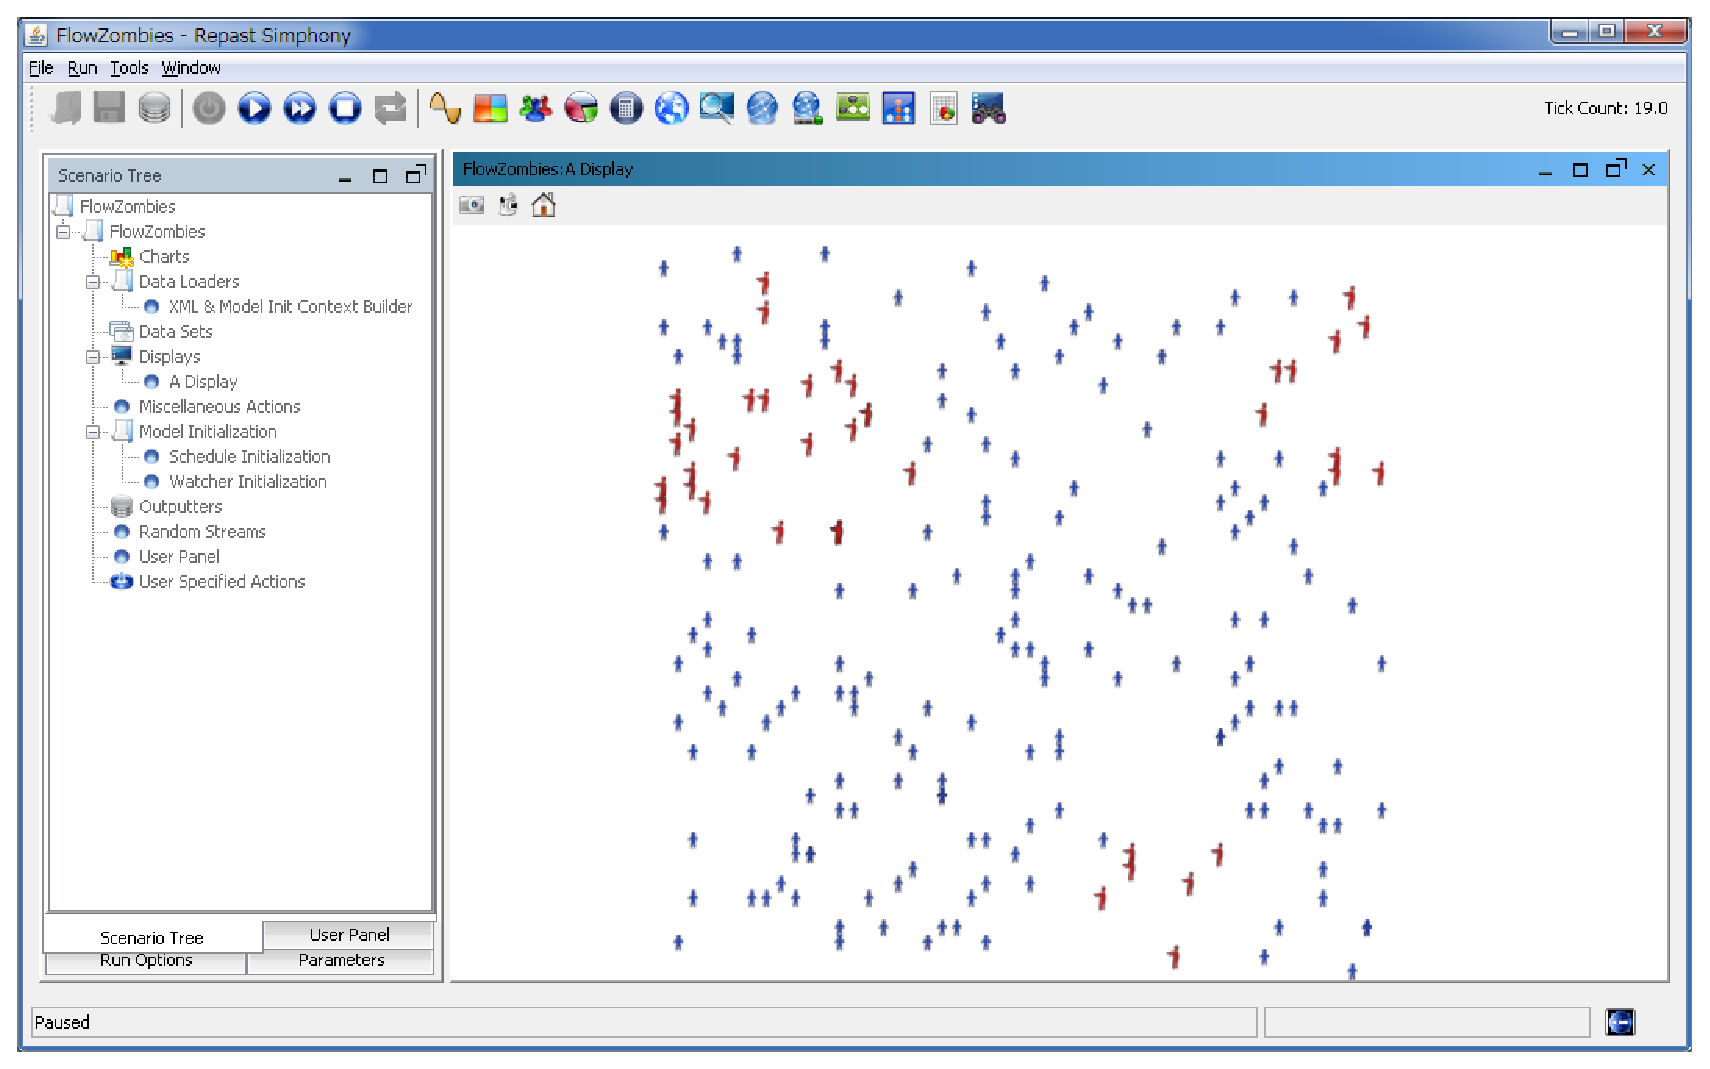
\includegraphics[width=5in]{figs/final.eps}
}
\caption{Completed Zombies Model}
\label{fig:final}
\end{center}
\end{figure}

The first thing we must do is create a new Repast Simphony project. Assuming you've started Repast Simphony, right click in the Package Explorer pane and choose ``New'' then ``Other''. A dialog box comes up that allows you to select a wizard. Select ``Repast Simphony Project'' under the ``Repast Simphony'' folder (Fig.~\ref{fig:newprojecticon}) and click ``Next''. This brings up the New Repast Simphony Project Wizard  which gives us the ability to name our project (and a few more options which we'll ignore for now). Type ``FlowZombies'' in the ``Project name" field, and press the ``Finish" button.

\begin{figure}[h]
\begin{center}
\vspace{.2in}
\centerline {
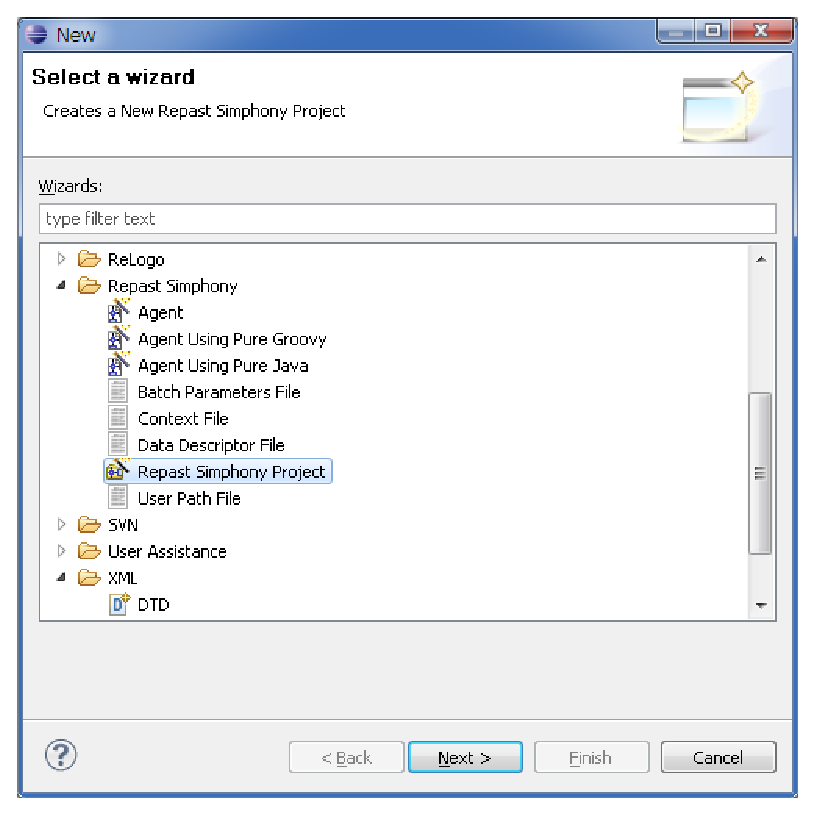
\includegraphics[width=3in]{figs/new_wizard.eps}
}
\caption{Repast Simphony Project Wizard.}
\label{fig:newprojecticon}
\end{center}
\end{figure}

By default Repast Simphony will hide many of the details of the project. This is appropriate for ReLogo projects but not for those written with Flowcharts or in Java. If the ReLogo filters have not been previously disabled then we need to do that now. If you click on the ``+'' (Windows) or triangle (OSX) next to ``FlowZombies'' and you see a variety of folders (batch, docs, etc), then the filter has been disabled. If you only see the src directory then the filter needs to be disabled. To disable the filter, click the downward pointing arrow in the ``Package Explorer'' pane. If you see ``ReLogo Resource Filter''  then click on it to disable the filter (Fig.~\ref{fig:filter}).  Otherwise, click on the ``Filters'' item. This brings up the Java Element Filters windows. Scroll through the elements and click off the checkbox for ReLogo Resource Filter (Fig.~\ref{fig:filter2}). 

\begin{figure}[h]
\begin{center}
\vspace{.2in}
\centerline {
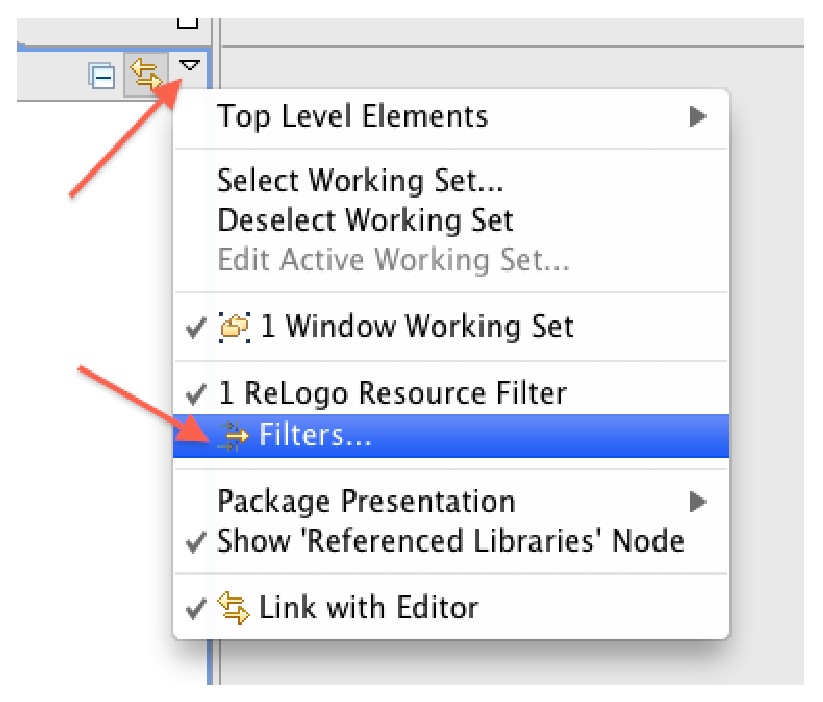
\includegraphics[width=3in]{figs/filter.eps}
}
\caption{Disabling the ReLogo Filter.}
\label{fig:filter}
\end{center}
\end{figure}


\begin{figure}[h]
\begin{center}
\vspace{.2in}
\centerline {
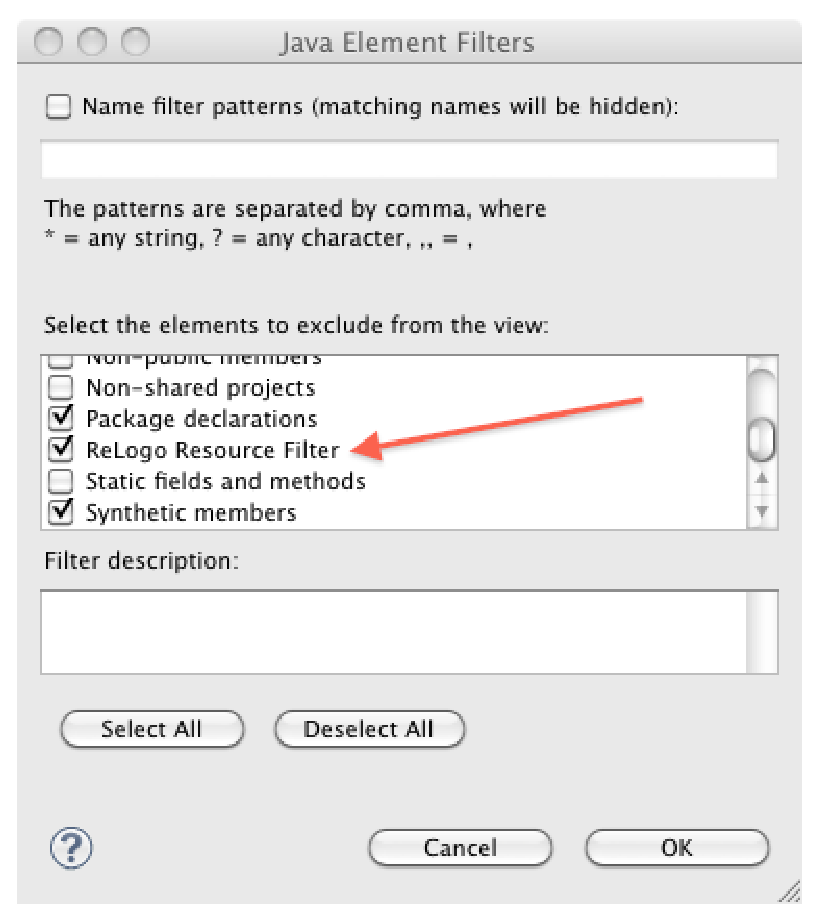
\includegraphics[width=3in]{figs/filter_window.eps}
}
\caption{Filter Window.}
\label{fig:filter2}
\end{center}
\end{figure}

In addition, by default autobuilding is disabled. However, this is not appropriate for projects written with Flowcharts and in Java. To enable auto building go to the Project menu and select Build Automatically.

Lastly, if Eclipse has defaulted to the ReLogo perspective switch it to the Java one. The perspective selections can be found in the upper right hand corner (Fig.~\ref{fig:javap}). Click the Java perspective.

\begin{figure}[h]
\begin{center}
\vspace{.2in}
\centerline {

\includegraphics[width=3in]{figs/perspectives.eps}
}
\caption{Selecting the Java Perspective.}
\label{fig:javap}
\end{center}
\end{figure}

\subsection{Building the Model}
Repast agents may be created through several different paths, such as pure Java agents, Groovy agents, or Flowchart agents.  This tutorial will demonstrate agent design using the Flowchart method.  The Repast Simphony project wizard creates a source directory and default package into which we can create these agent classes. In our case, the package is ``FlowZombies'', which can be seen immediately under the src directory.\footnote{Package names typically use an internet domain name as the basis for a package name, but for the purposes of this tutorial ``FlowZombies'' is perfectly fine. See  \href{http://download.oracle.com/javase/tutorial/java/package/namingpkgs.html}{Java Tutorial: packages} for more info.} 

To create a new Flowchart agent, right click on the created ``FlowZombies'' package located in the newly create project.  Select ``New'', then ``Other'' and browse to the ``Repast Simphony'' category (Fig.~\ref{fig:newagent1}).  Select ``Agent'' and in the File name, rename the default ``Untititled.agent'' to ``Human.agent'' (Fig.~\ref{fig:newagent2}).  Repeat this process for the Zombie agent, using the name ``Zombie.agent''. 

\begin{figure}[h]
\begin{center}
\vspace{.2in}
\centerline {
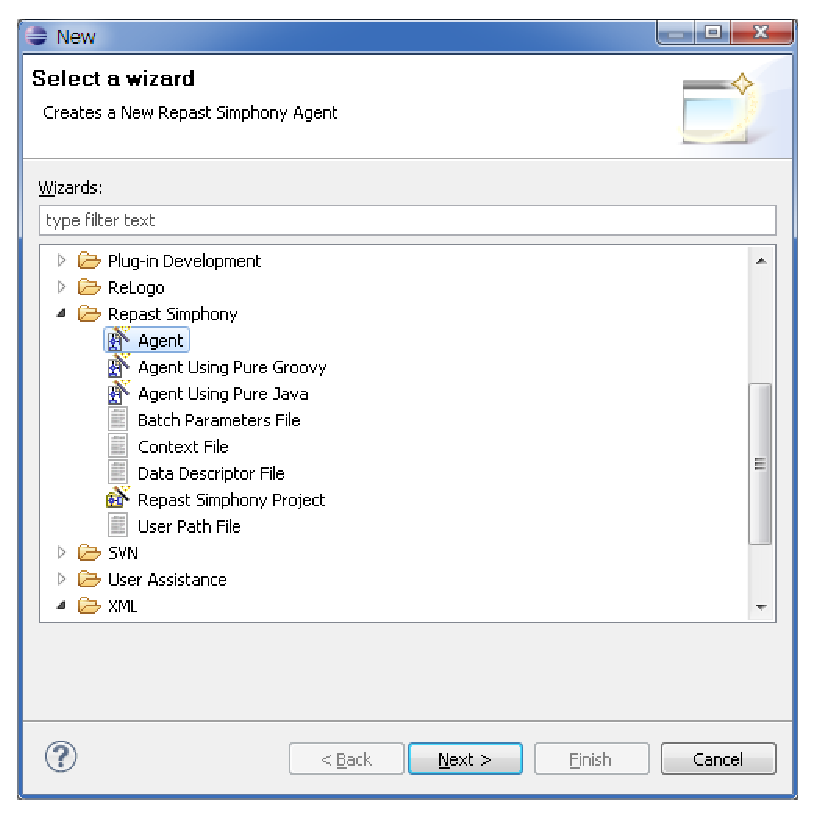
\includegraphics[width=3in]{figs/newAgentWiz_1.eps}
}
\caption{New Agent Wizard Step 1}
\label{fig:newagent1}
\end{center}
\end{figure}

\begin{figure}[h]
\begin{center}
\vspace{.2in}
\centerline {
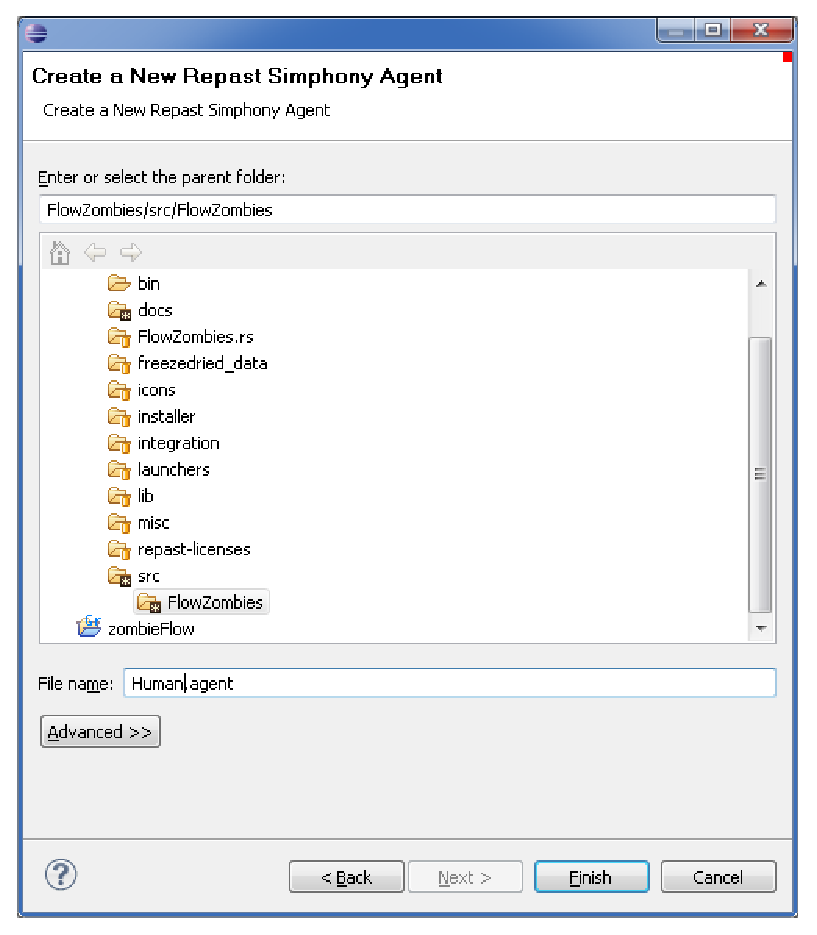
\includegraphics[width=3in]{figs/newAgentWiz_2.eps}
}
\caption{New Agent Wizard Step 2}
\label{fig:newagent2}
\end{center}
\end{figure}

The \texttt{Zombie.agent}  and \texttt{Human.agent} files (along with the automatically generated \texttt{Zombie.groovy}  and \texttt{Human.groovy} files) should be visible in the FlowZombies packages underneath the src folder, and the Agent flowcharts should be open in Eclipse's editor pane. (If ihey are not open, double click on each \texttt{Human.agent} file to open it). Let's begin with the Zombies. The Zombies behavior is to wander around looking for Human's to infect. More specifically, each iteration of the simulation, each Zombie will determine where the most Humans are within its local area and move there. Once there it will attempt to infect a Human at that location and turn it into a Zombie. 

We will begin by implementing the movement. To do this we will locate the Zombies and Humans within a \texttt{Grid}. The \texttt{Grid} allows us to do neighborhood and proximity queries (i.e. ``who is near me?'') using discrete integer Grid coordinates.\footnote{More details on \texttt{Grid} can found in the Repast Java API documentation and the Repast Reference.} Let's begin by adding a property to the Zombie Agent that indicates whether the Zombie has moved.  To create a Property block in the Flowchart, click on the Property icon the the Steps pane and then click on the Flowchart canvas.  The Property block will appear and may be selected.  Selecting an element in a flowchart allows the element to be edited using the Properties pane at the bottom of the window.  If the Properties pane is not visible, right click on a flowchart element and select ``Show Properties.''

Select the Moved Property and in the Properties pane, enter the following information:

\begin{enumerate}
\item Step 2: Moved
\item Step 3: moved
\item Step 5: boolean
\item Step 6: false
\end{enumerate}

This initial flowchart should look like Fig.~\ref{fig:zombie1}. Now lets add a Behavior to Zombie that will be executed every iteration of the simulation.  Select a new Behavior block from the Steps pane in the flowchart editor and add it to the flowchart (Fig.~\ref{fig:zombie2}).  In the properties pane, edit the following items for this Behavior:

\begin{enumerate}
\item Step 3a: Type in a Constant Starting Time for the Behavior : 1
\item Step 3c: Type in a Constant Repeat Interval for the Behavior: 1
\end{enumerate}

Next, we will provide details for all elements of the movement Behavior.  The completed flowchart for this behavior is shown in figure (Fig.~\ref{fig:zombie3}).  Add the various blocks from the Steps pane so that it looks like the completed flowchart  in Fig.~\ref{fig:zombie3}. Connections between the step blocks can be created by choosing the ``Connection'' option in the flow chart editor, clicking on a step block and dragging to the other. Once the flowchart steps and connections have been added, we will now proceed to edit each of the flowchart elements. 

Task Grid Neighbors
\begin{enumerate}
 \item Grid grid = FindGrid("FlowZombies/grid")
 \item GridPoint pt = grid.getLocation(this)
 \item GridCellNgh nghCreator = new GridCellNgh(grid, pt, Human.class, 1, 1)
 \item List gridCells = nghCreator.getNeighborhood(true)
 \item SimUtilities.shuffle(gridCells, RandomHelper.getUniform())
\end{enumerate}

Task Initialize loop
\begin{enumerate}
 \item GridPoint pointWithMostHumans = null
 \item int maxCount = -1
\end{enumerate}

Loop over neighbors
\begin{enumerate}
 \item Step 3: GridCell cell in gridCells
\end{enumerate}

Decision Check count
\begin{enumerate}
 \item Step 3: cell.size() $>$ maxCount
\end{enumerate}

Task Point with most humans
\begin{enumerate}
 \item pointWithMostHumans = cell.getPoint()
 \item maxCount = cell.size()
\end{enumerate}

Task Move and Infect
\begin{enumerate}
 \item int x = pointWithMostHumans.getX()
 \item int y = pointWithMostHumans.getY()
 \item grid.moveTo(this,x,y)
 \item moved = true
 \item infect()
\end{enumerate}

Finally, we need to define the Infect behavior for the Zombie agent.  The completed flowchart for the agent is shown in (Fig.~\ref{fig:zombieComplete}).

Behavior Infect
\begin{enumerate}
 \item Step 7: Type in a Compiled Name : infect
\end{enumerate}

Task Find Humans
\begin{enumerate}
 \item Grid grid = FindGrid("FlowZombies/grid")
 \item GridPoint pt = grid.getLocation(this)
 \item List humans = new ArrayList()
 \item Iterable objects = grid.getObjectsAt(pt.getX(), pt.getY())
\end{enumerate}

Loop over objects
\begin{enumerate}
 \item Step 3: objects.hasNext()
\end{enumerate}

Task Get Object
\begin{enumerate}
 \item Object o = objects.next()
\end{enumerate}

Decision is Human?
\begin{enumerate}
 \item Step 3: o instanceof Human
\end{enumerate}

Task save human
\begin{enumerate}
 \item humans.add(o)
\end{enumerate}

Decision Found Humans?
\begin{enumerate}
 \item Step 3: humans.size() $>$ 0
\end{enumerate}

Task Braaaaaains!
\begin{enumerate}
 \item int index = RandomHelper.nextIntFromTo(0, humans.size() - 1)
 \item Object human = humans.get(index)
 \item Context context = RemoveAgentFromContext("FlowZombies", human)
 \item Object zombie = CreateAgents("FlowZombies", "FlowZombies.Zombie", 1)
 \item MoveAgent("FlowZombies/grid", zombie, pt.getX(), pt.getY())
\end{enumerate}

\begin{figure}[p]
\begin{center}
\vspace{.2in}
\centerline {
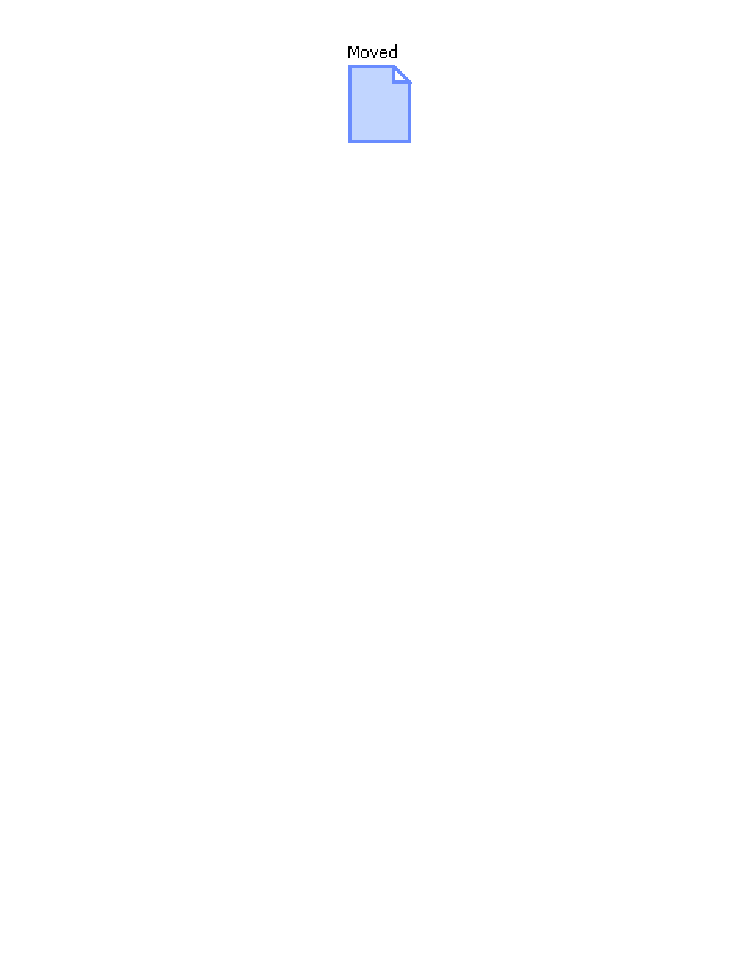
\includegraphics[width=3in]{figs/Zombie_1.eps}
}
\caption{Zombie Agent Step 1}
\label{fig:zombie1}
\end{center}\end{figure}

\begin{figure}[p]
\begin{center}
\vspace{.2in}
\centerline {
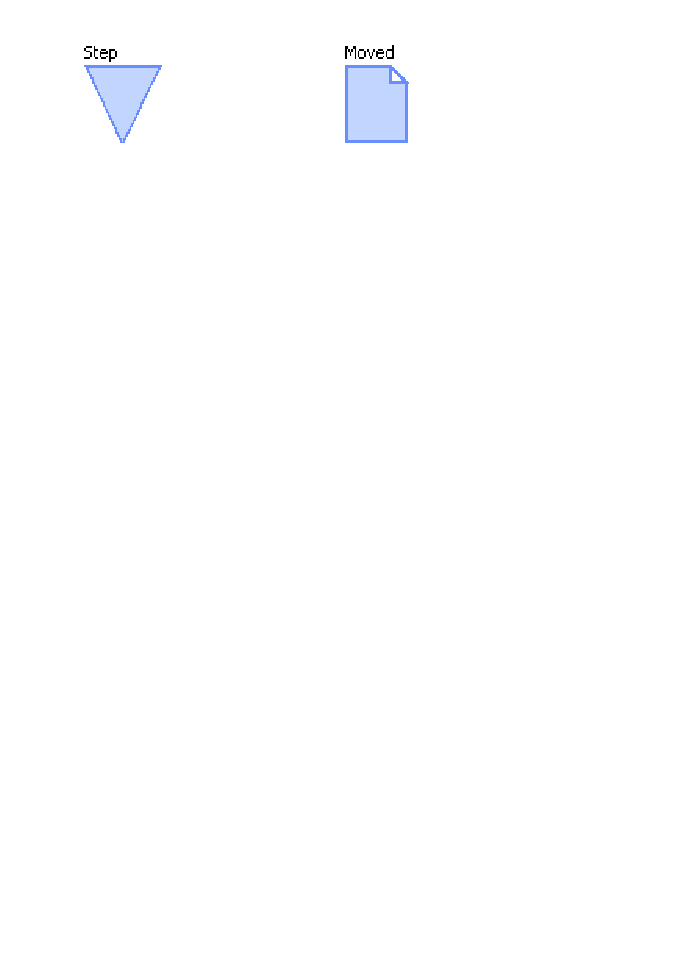
\includegraphics[width=3in]{figs/Zombie_2.eps}
}
\caption{Zombie Agent Step 2}
\label{fig:zombie2}
\end{center}
\end{figure}

\begin{figure}[p]
\begin{center}
\vspace{.2in}
\centerline {
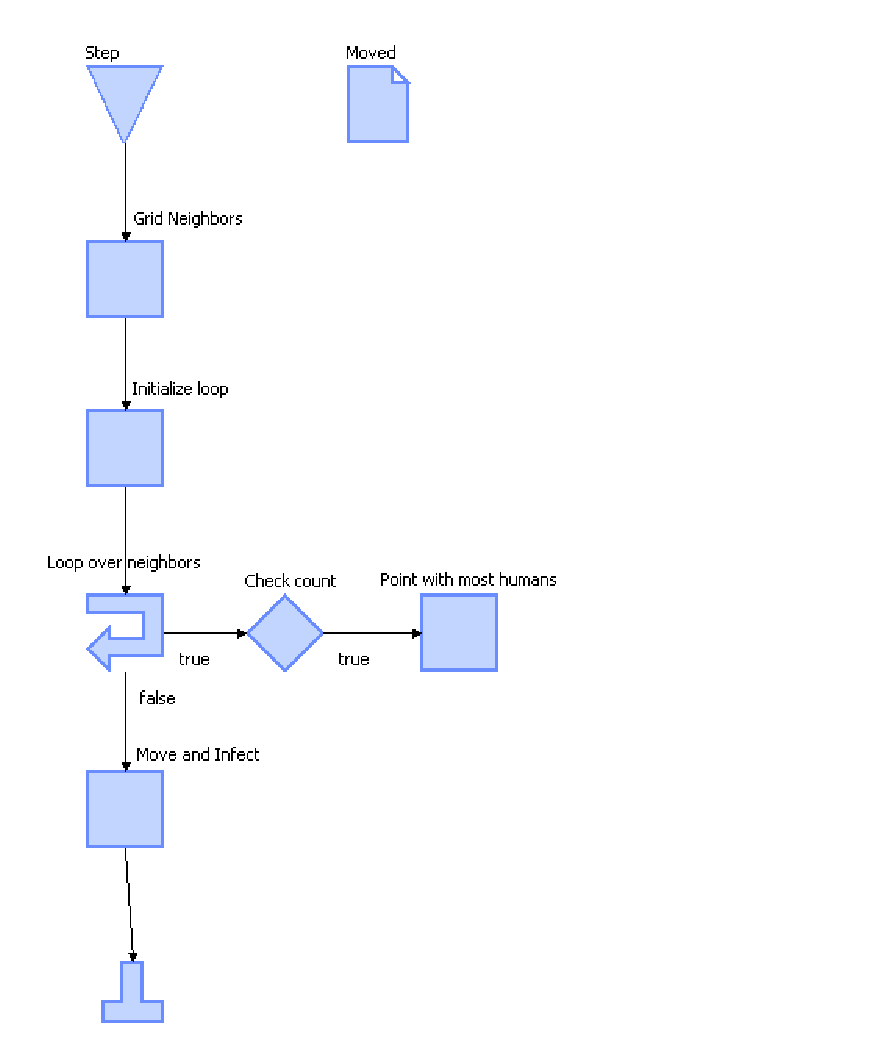
\includegraphics[width=3in]{figs/Zombie_3.eps}
}
\caption{Zombie Agent Step 3}
\label{fig:zombie3}
\end{center}
\end{figure}

\begin{figure}[p]
\begin{center}
\vspace{.2in}
\centerline {
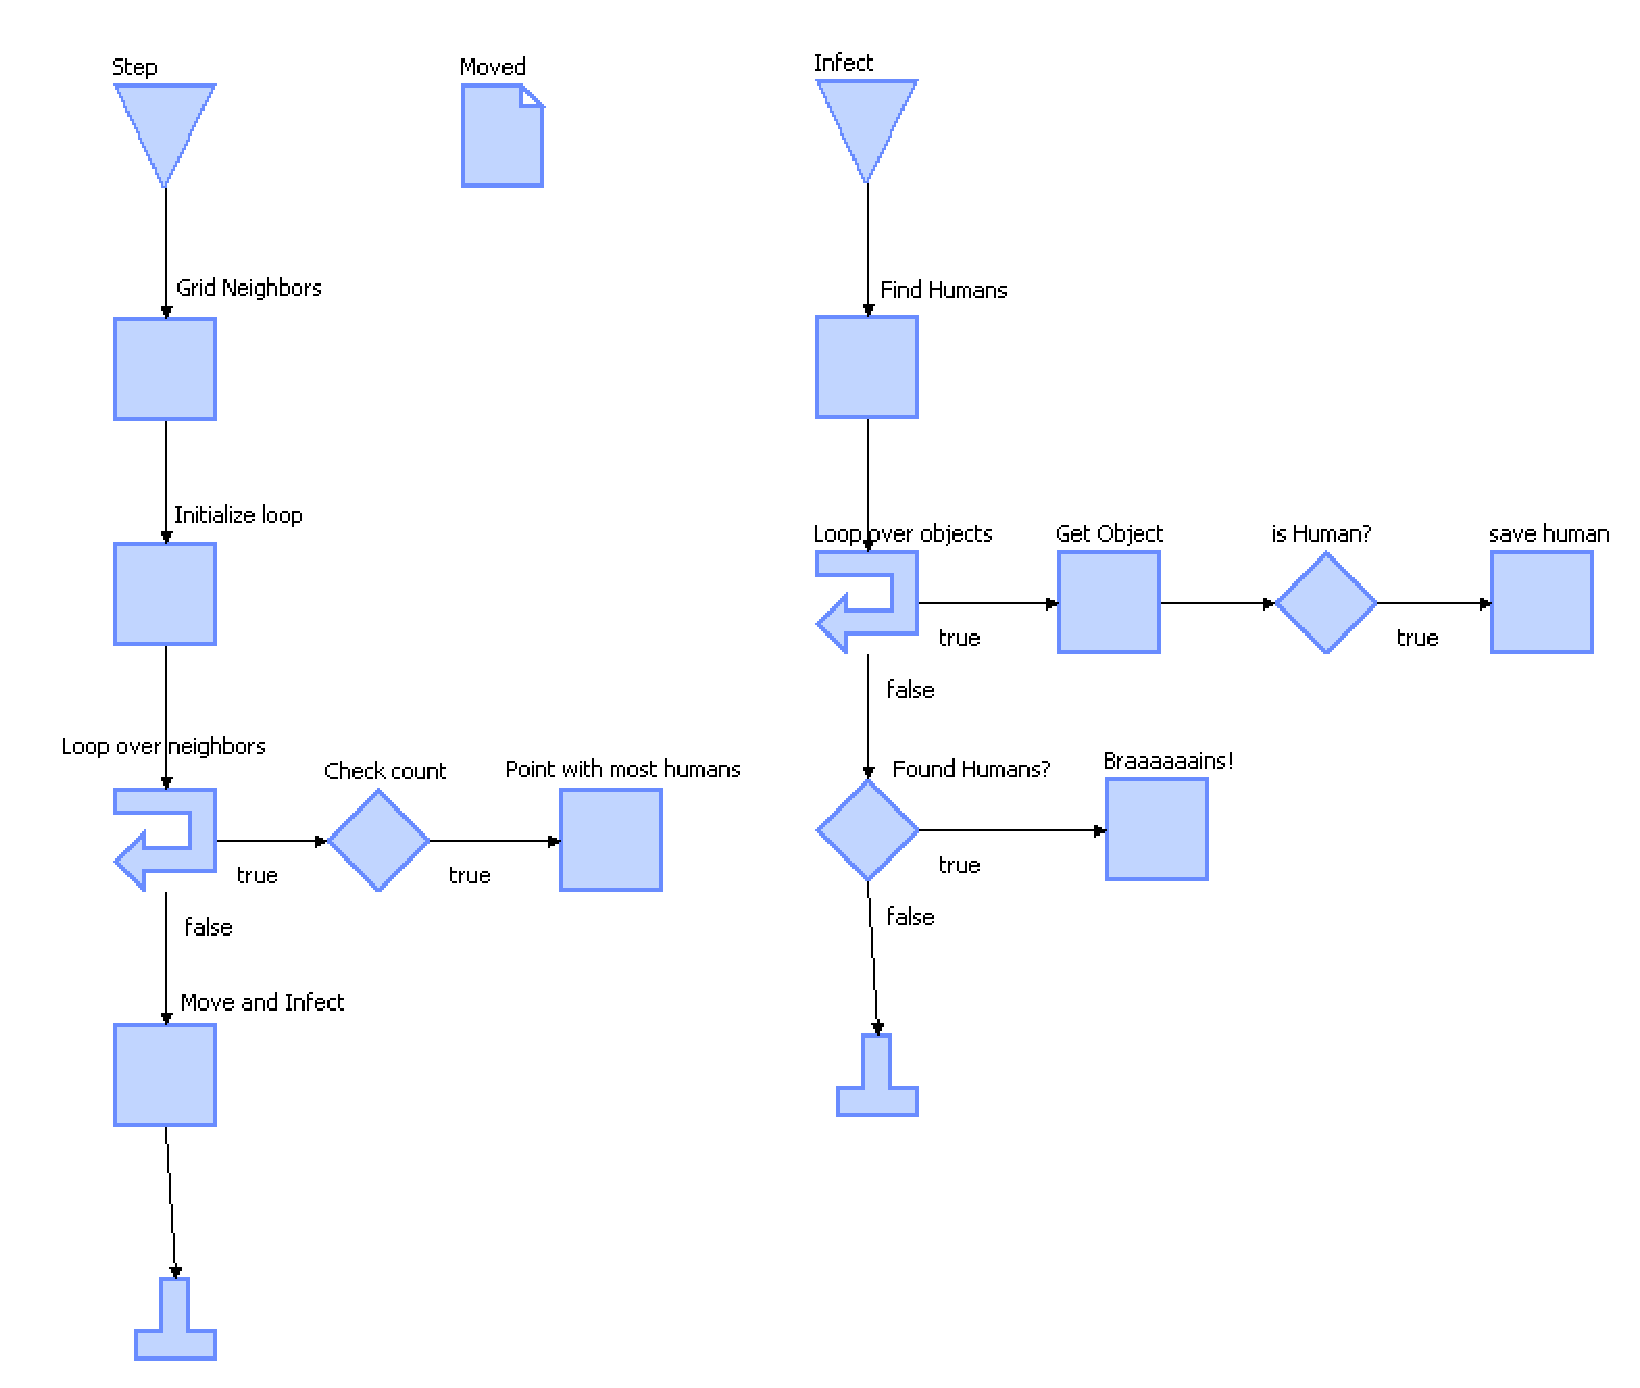
\includegraphics[width=3in]{figs/Zombie_complete.eps}
}
\caption{Zombie Agent Completed}
\label{fig:zombieComplete}
\end{center}
\end{figure}

\FloatBarrier

Let's now turn to the code for the Humans. Select Human.agent in Eclipse's editor pane. The basic behavior for a Human is to react when a Zombie comes within its local neighborhood by running away from the area with the most Zombies. Additionally, Humans have  a certain amount of energy that is expended in running away. If this energy is 0 or less then a Human is unable to run. We begin by creating properties of \texttt{Energy} and \texttt{Starting Energy}. \texttt{Energy} will be used to track the current amount of energy a Human has.  \texttt{Starting Energy} will be used to set the energy level back to its starting level after a Human has had a rest.  The main behavior of a Human is implemented in its \texttt{run} Behavior.  The starting point for the Human flowchart is shown in (Fig.~\ref{fig:humanstart})  Create the properties for Energy and Starting Energy and create the Run Behavior.

Property Energy
\begin{enumerate}
 \item Step 2: Energy
 \item Step 3: energy 
 \item Step 5: int
 \item Step 6: 10
\end{enumerate}

Property Start Energy
\begin{enumerate}
 \item Step 2: Start Energy
 \item Step 3: startEnergy
 \item Step 5: int
 \item Step 6: 10
\end{enumerate}

Behavior Run
\begin{enumerate}
 \item Step 4b: Type in a Query for the Trigger Condition : within\_vn 1
 \item Step 4c: Type in Kind of Agents to Watch : FlowZombies.Zombie
 \item Step 4d: Type in a Comma Separated List of Target Agent Fields To Watch : moved
 \item Step 4f: Type in a Delay Kind Before the Behavior Triggers : Immediate
 \item Step 4g: Type in a Delay Time Before the Behavior Triggers : 0   
\end{enumerate}

Next, we will provide the mechanism for the Run Behavior.  Fig.~\ref{fig:humanstart} shows the completed Human flowchart.  Enter the details for each of the following flowchart blocks:

Task Grid Neighbors
\begin{enumerate}
 \item Grid grid = FindGrid("FlowZombies/grid")
 \item GridPoint pt = grid.getLocation(this)
 \item GridCellNgh nghCreator = new GridCellNgh(grid, pt, Zombie.class,1,1)
 \item List gridCells = nghCreator.getNeighborhood(true)
 \item SimUtilities.shuffle(gridCells, RandomHelper.getUniform())
\end{enumerate}

Task Initialize loop
\begin{enumerate}
 \item GridPoint pointWithLeastZombies = null
 \item int minCount = Integer.MAX\_VALUE
\end{enumerate}

Loop over neighbors
\begin{enumerate}
 \item Step 3: GridCell cell in gridCells
\end{enumerate}

Decision check count
\begin{enumerate}
 \item cell.size() $<$ minCount
\end{enumerate}

Task Point with least zombies
\begin{enumerate}
 \item pointWithLeastZombies = cell.getPoint()
 \item minCount = cell.size()
\end{enumerate}

Decision Check energy
\begin{enumerate}
 \item Step 3: energy $>$ 0
\end{enumerate}

Task Move
\begin{enumerate}
 \item int x = pointWithLeastZombies.getX()
 \item int y = pointWithLeastZombies.getY()
 \item grid.moveTo(this,x,y)
 \item energy$--$
\end{enumerate}

Task Reset Energy
\begin{enumerate}
 \item energy = startingEnergy
\end{enumerate}


\begin{figure}[p]
\begin{center}
\vspace{.2in}
\centerline {
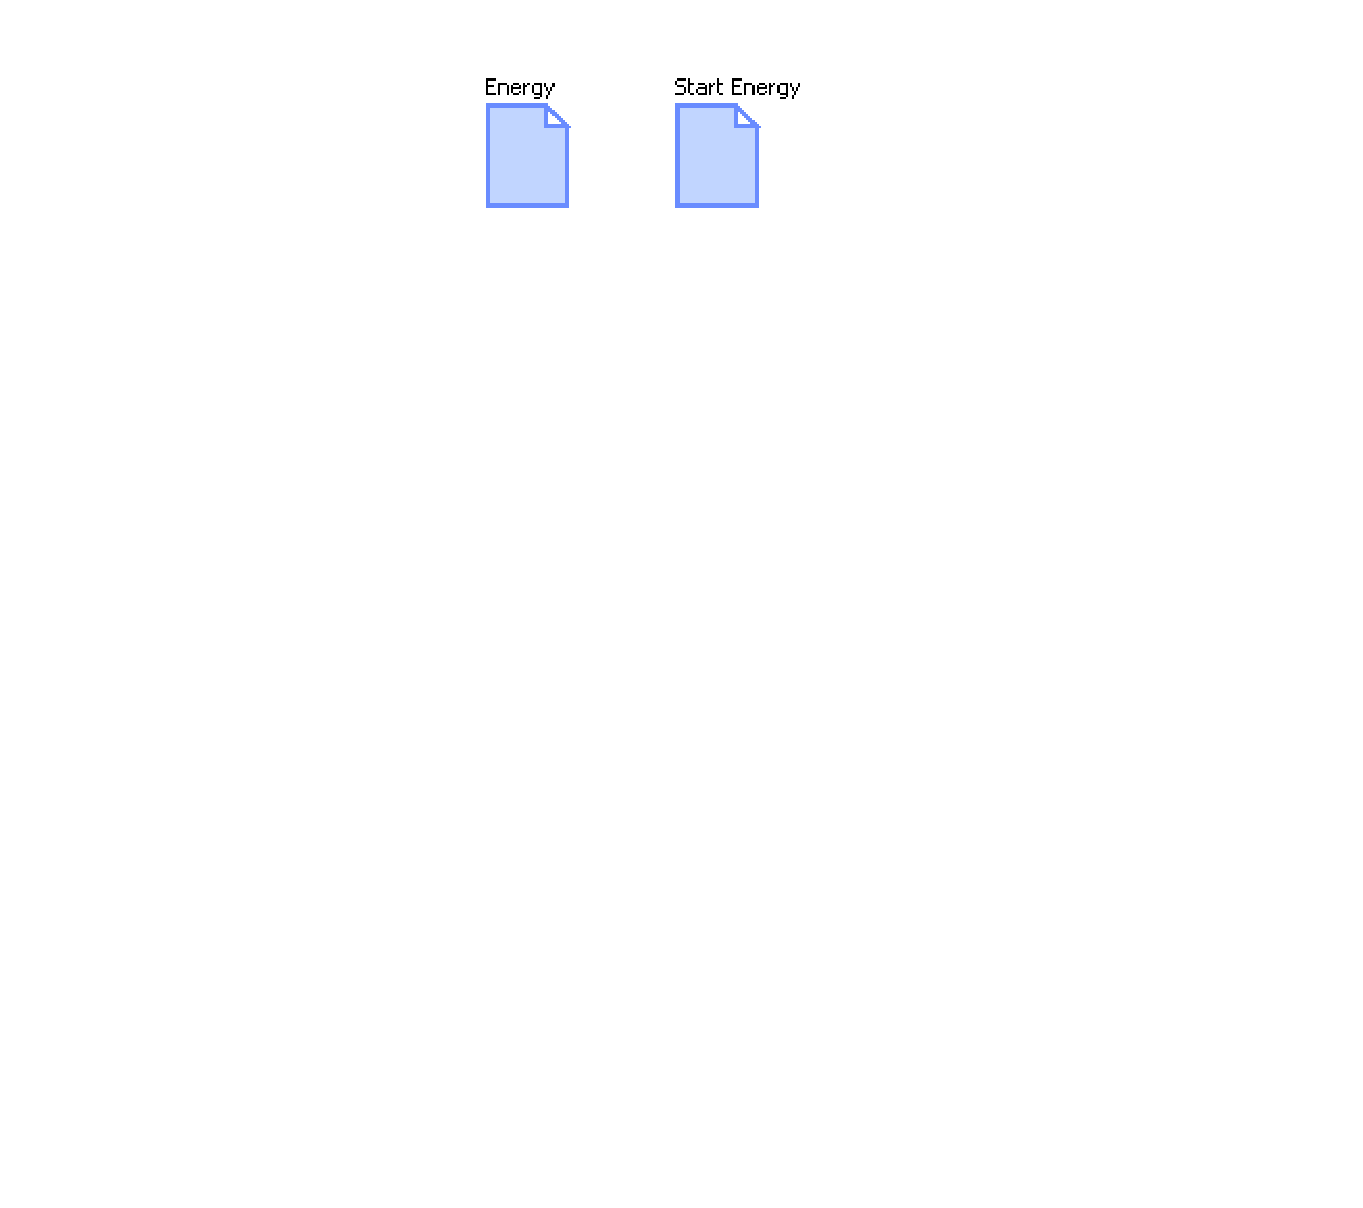
\includegraphics[width=3in]{figs/Human_start.eps}
}
\caption{Human Agent Start}
\label{fig:humanstart}
\end{center}\end{figure}

\begin{figure}[p]
\begin{center}
\vspace{.2in}
\centerline {
\includegraphics[width=3in]{figs/Human_complete.eps}
}
\caption{Human Agent Completed}
\label{fig:humancomplete}
\end{center}\end{figure}

\FloatBarrier

This looks much like the Zombie code. A \texttt{GridCellNgh} is used to find the Zombies in the neighboring grid cells. It then determines which of these cells has the least Zombies and attempts to move towards that. Note that \texttt{moveTo} is only called if the energy level is greater than 0. If energy does equal 0, the Human doesn't move and energy is set back to its starting level.  Unlike the Zombie code we are not going to schedule the \texttt{run()} method for execution. Rather we are going to setup a \textit{watcher} that will trigger this run() method whenever a Zombie moves into a Human's neighborhood.  The watcher will trigger whenever this field has been accessed.

This \texttt{Watch} will watch for any changes to a ``moved" property in the Zombies agent. What this means is whenever any Zombie moves and their moved variable is updated, then this \texttt{Watch} will be checked for each Human. If the query returns true for that particular Human then \texttt{run} will be called immediately on that Human. Our query will return true when the Zombie that moved is within the Moore neighborhood (8 surrounding grid cells) of the Human whose \texttt{Watch} is currently being evaluated.

That completes this part of the code for Zombies and Humans. Now we need to turn to initializing the simulation which is achieved with a special type of agent called the ``ModelInitializer.''  The ModelInitializer agent is used to hold actions done during the simulation initialization, such as creating agents.  Create the ModelInitializer agent in the same way as was done with the Human and Zombie agents through the new agent wizard.  It is important that the agent name is exactly ``ModelInitializer'' as Repast will look for this specifically named agent.  

First, create a behavior in the ModelInitializer that will start the initialization process.  This is a behavior step that will occur only one time at the very beginning of the simulation.

Behavior Initialize Model
\begin{enumerate}
 \item Step 2: Initialize Model
 \item Step 4f: Immediate 
 \item Step 7: initializeModel
\end{enumerate}

Note that in Step 7 it is important that the property value is exactly ``initializeModel'' as this is a special property name used by the ModelInitializer agent.  Create an End step and connect as shown in Fig.~\ref{fig:mistart}. This initialize behavior and end step are the mimimum required steps in the ModelInitializer to create a runnable simulation.  Without these steps, an error will be produed when the model is initialzed.  Of course, the model inizialzer behavior is still empty so we need to add steps to create the Human and Zombie models.

We will create a specified number of Zombies and Humans by looping through some creation code a specified number of times. We then add the new Zombies and Humans to context. In adding them to the context we automatically add them to any projections associated with that context.  The completed Model Initializer agent is shown in Fig.~\ref{fig:micomplete}.

Property Human Count
\begin{enumerate}
 \item Step 2: Human Count
 \item Step 3: humanCount 
 \item Step 5: int
 \item Step 6: 200
\end{enumerate}
 
Property Zombie Count
\begin{enumerate}
 \item Step 2: Zombie Count
 \item Step 3: zombieCount 
 \item Step 5: int
 \item Step 6: 5
\end{enumerate}

Loop Count Humans
\begin{enumerate} 
 \item Step 3: i in 1..humanCount
\end{enumerate}

Task Create Humans
\begin{enumerate}
 \item Object agent = CreateAgents(``FlowZombies'', ``FlowZombies.Human'',1)
 \item Human human = (Human)agent
 \item  human.energy = RandomHelper.nextIntFromTo(4, 10)
 \item  human.startEnergy = human.energy
\end{enumerate}

Task Create Zombies
\begin{enumerate}
 \item CreateAgents(''FlowZombies'', ``FlowZombies.Zombie'',zombieCount)
\end{enumerate}

\begin{figure}[p]
\begin{center}
\vspace{.2in}
\centerline {
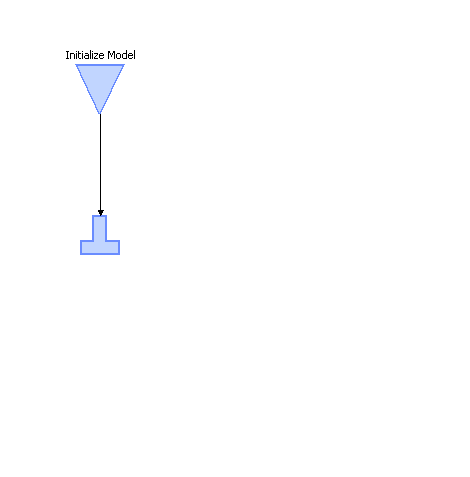
\includegraphics[width=3in]{figs/ModelInitializer_start.png}
}
\caption{Model Initializer Start}
\label{fig:mistart}
\end{center}
\end{figure}

\begin{figure}[p]
\begin{center}
\vspace{.2in}
\centerline {
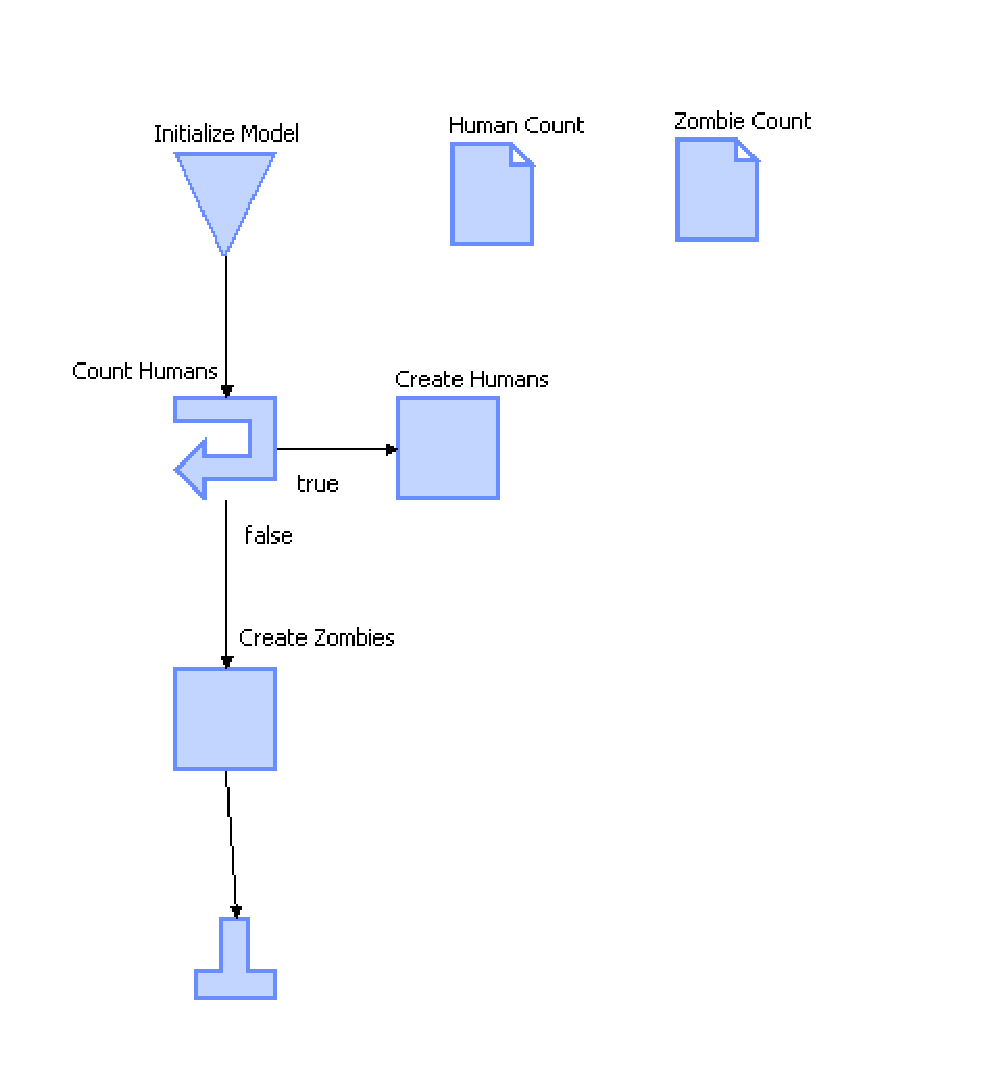
\includegraphics[width=3in]{figs/ModelInitializer_complete.eps}
}
\caption{Model Initializer Completed}
\label{fig:micomplete}
\end{center}
\end{figure}

\FloatBarrier

Before we run this model, we need to update the metadata that the Repast Simphony runtime uses to help create displays and other runtime components. Open the FlowZombies.rs folder under the project folder, and double click on the \texttt{context.xml} file.

That should bring up the xml editor for editing the \texttt{context.xml} file. The \texttt{context.xml} file describes the context hierarchy for your model. The context hierarchy is composed of the contexts your model uses and the projections associated with them. 

We need to add a Grid projection using the editor.  To do that, 
\vspace{.2in}
\begin{enumerate}
\item Right click on the context element and select ``Add Child'', then choose ''projection''.
\item Expand the projection element by clicking on the triangle next to the newly added projection.
\item Choose ``grid'' from the drop down box to set the value of the type attribute
\item Type ``grid'' (no quotes) for the id of the projection.
\item Right click on the new projection element and select select ``Add Child'', then choose ''attribute''.
\item Expand the attribute and set its id, type and value properties to width, int, and 50 respectively.
\item Add another attribute to the projection and set its id, type and value properties to height, int, and 50.
\item Add another attribute to the projection and set its id, type, and value properties to border rule, string, periodic.
\item Add another attribute to the projection and set its id, type, and value properties to allows multi, boolean and true.
\end{enumerate}

The context.xml editor should now look like Fig.~\ref{fig:context}.

\begin{figure}[h]
\begin{center}
\vspace{.2in}
\centerline {
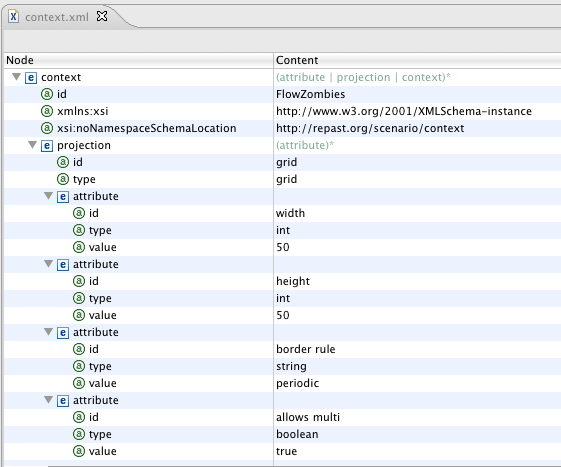
\includegraphics[width=3in]{figs/context.png}
}
\caption{context.xml location}
\label{fig:context}
\end{center}
\end{figure}

Now its time to launch the model. When we created our project using the Repast Simphony Project Wizard, it automatically created Eclipse launchers for us, and we can use those to launch the model. If you click on the small downward facing triangle next to the Eclipse launcher button (fig.~\ref{fig:launch}), you'll see the various available launchers. Click on ``FlowZombies Model''.

\begin{figure}[h]
\begin{center}
\vspace{.2in}
\centerline {
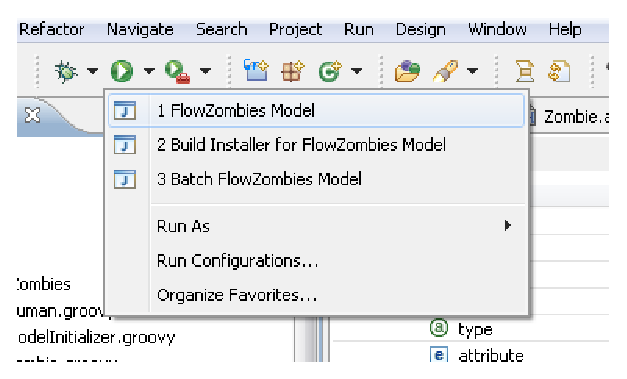
\includegraphics[width=3in]{figs/launcher.eps}
}
\caption{FlowZombies Model Launcher}
\label{fig:launch}
\end{center}
\end{figure}

When the model window appears, we can observe the Scenario Tree on the left hand side of the window.  The Scenario Tree allows us to customize things like model initialization, data logging, and displays.  We first need to specify how the model is initialized and we will do so with the ModelInitializer agent we created.  In the Scenario Tree right click on the Data Loaders and select ``Set Data Loader.''  A list appears with the various types of data loading options available.  Select ``Context.xml file and ModelInitializer'' and then click Next and Finish.

Next, we will now create a simple display. 

\vspace{.2in}
\begin{enumerate}
\item Right click on Displays in the Scenario Tree and click ``Add Display''
\item In the Display configuration dialog, type Grid Display for name. Leave 2D as the type.
\item Select our ``grid'' projection as the one we want to display. Click on space in the ``Projection and Value Layers'' section and then click the green arrow. The projections on the right are the ones will be displaying and those on the left are all the possible projections to display. The dialog should now look like fig.~\ref{fig:disp1}
\item Click Next.
\item Select the Human and Zombie agents as the types we want to display. Do this by selecting each in the left and then clicking the right pointing arrow to move them to right. If Zombie is not at the top of the list on the left use the up and down arrows to move it to the top. The dialog should now look like fig.~\ref{fig:disp2}
\item Click Next.
\item In this panel, we can configure what we want the Zombies and Humans to look like. This can be done programmatically by specifying a class that implements \texttt{repast.simphony.visualizationOGL2D.StyleOGL2D} or via a wizard. At this point you have two options, you can use the icons from the completed FlowZombies model to represent your agents or use a simpler style. We present the simpler style first.
\item Simple Style
\begin{enumerate}
\item Click the button to the right of the style class combo box (fig.~\ref{fig:disp3}).
\item In the 2D Shape editor, change the Icon Shape to a square using the combo box and change the color to red by clicking the button with the blue square, and choosing a red color from the icon color dialog. Click OK on the icon color box, then OK on the 2D Shape Editor.
\item Repeat the previous step for the Human. Click on Human in the list of Agents. Then click the icon editor button as before. Leave the default as is, and click OK. 
\end{enumerate}
\item Icon Style
\begin{enumerate}
\item Click the button to right of the style class combo box (fig.~\ref{fig:disp3}).
\item In the 2D Shape editor, click on the ``Select Icon File'' button. We want to use the zombie.png icon that comes with the jzombies demo model. Navigate to where the demo models are installed and click on zombies.png in the \texttt{jzombies/icon} directory. (If you can't find zombies.png, feel free to style the Zombie as a circle or whatever, using the 2D Shape editor).
\item Click OK when you have finished.
\item Repeat the previous step for the Human. Click on Human in the list of Agents. Then click the icon editor button as before. Click the``Select Icon File'' button and navigate to the \texttt{jzombies/icon} directory in the demo model. Choose the person.png icon.
\item Click OK when you have finished with the 2D Shape editor.
\end{enumerate}

\item Click Next
\item Click Next
\item Click Finish
\end{enumerate}
\vspace{.2in}

\begin{figure}[h]
\begin{center}
\vspace{.2in}
\centerline {
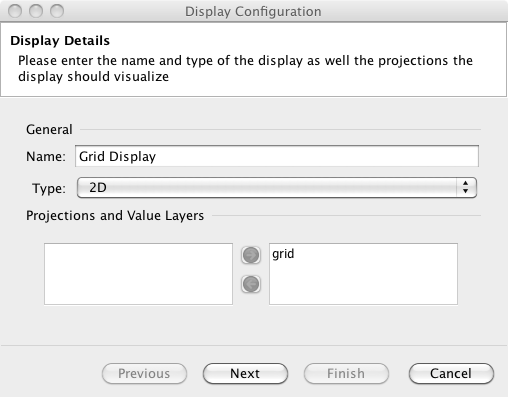
\includegraphics[width=3in]{figs/display1.png}
}
\caption{Configuring the Display}
\label{fig:disp1}
\end{center}
\end{figure}

\begin{figure}[h]
\begin{center}
\vspace{.2in}
\centerline {
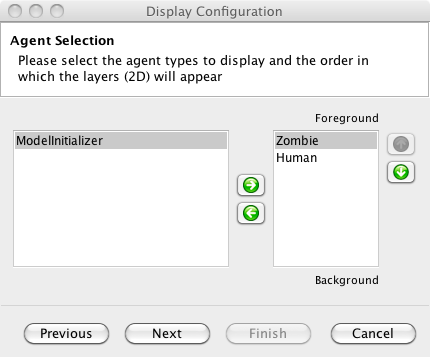
\includegraphics[width=3in]{figs/display2.png}
}
\caption{Configuring the Display 2}
\label{fig:disp2}
\end{center}
\end{figure}

\begin{figure}[h]
\begin{center}
\vspace{.2in}
\centerline {
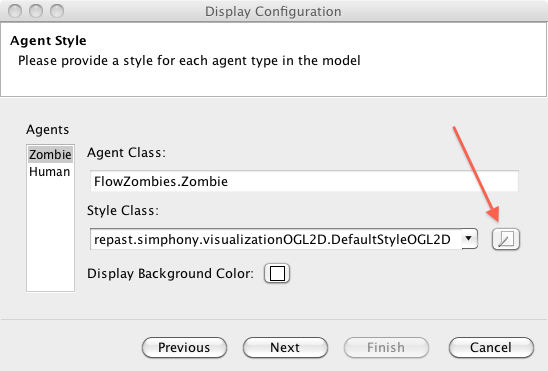
\includegraphics[width=3in]{figs/display3.png}
}
\caption{Configuring the Display 3}
\label{fig:disp3}
\end{center}
\end{figure}

You should now see ``Grid Display'' under the Display node in the Scenario Tree. Save your new scenario info (the new Data Loader and Display) by clicking the ``Save'' button (fig.~\ref{fig:save_button}) on the Repast Simphony runtime toolbar.

\begin{figure}[h]
\begin{center}
\vspace{.2in}
\centerline {

\includegraphics[width=3in]{figs/save_button.eps}
}
\caption{Save Scenario Button}
\label{fig:save_button}
\end{center}
\end{figure}


We can now run our model. Click the Initialize button (fig.~\ref{fig:buttons}) to initialize the model and bring up the display. If the display is not centered, you can center it by clicking on the display ``home'' button to reset the view. The mouse wheel will zoom the display in and out as will holding down the shift key and right mouse button and moving the mouse up and down. You can run the simulation by clicking the Run button, step through each timestep with the Step button, stop the simulation with the Stop button, and reset it for another run with the Reset button (fig.~\ref{fig:buttons}). When the simulation has been stopped, you must reset it with the Reset button in order do any more runs.

\begin{figure}[h]
\begin{center}
\vspace{.2in}
\centerline {

\includegraphics[width=3in]{figs/buttons.eps}
}
\caption{Repast Simphony Simulation Buttons}
\label{fig:buttons}
\end{center}
\end{figure}

Once the Repast Simphony runtime has come up, initialize and run the simulation. You should now see humans becoming zombies. If you don't, then check your code for mistakes.

\subsection{Model Distribution}

Repast models can be distributed to model users via the installation builder. This feature packs up your model and all of the software you need to run it, except for a properly configured Java Runtime Environment, into a single Java archive ("JAR") file that can be given to model users. The resulting installer can be executed on any system with Java version 1.6 or later; JOGL; and Java3D installed\footnote{Users can obtain free JOGL and Java3D files from the Repast website downloads page \href{http://repast.sourceforge.net/downloads.html}{here}.}. Users simply copy the installer file onto their Windows, Mac OS, or Linux computers and the start the installer by double clicking on the file. Once the installer is started it will show an installation wizard that will prompt the user for the information needed to install the model. If desired, the installer can also be run in a command line mode.

Building an installer for a model is straightforward. Simply choose the ``Build Installer for $\langle$Your Model Name Here$\rangle$ Model'' and provide a location and name for the installer file. The installer file's default name is ``setup.jar,'' which is suitable for most purposes. The install builder will then package and compress your model and the supporting Repast software. The resulting installer files are about 70 MB plus the size of the model code and data. 75 MB to 80 MB is a common total size.

The Repast install builder uses the \href{http://izpack.org/}{IzPack system}.  More information on installer customization and use, including command line activation, can be found on the  \href{http://izpack.org/}{IzPack web site}.

\noindent\begin{minipage}[h]{\textwidth}
\vspace{.2in}
\lstset{language=java,caption=}
\begin{lstlisting}

\end{lstlisting}
\vspace{.2in}
\end{minipage}

\end{document}  
